\documentclass{article}
\usepackage[utf8]{inputenc}
\usepackage{graphicx}
\usepackage{hyperref}
\usepackage{amssymb}
\usepackage{amsmath}
\usepackage{graphicx}
\usepackage{algorithm2e}
\usepackage{algpseudocode}
\usepackage[english]{babel}
\usepackage{graphicx}
\usepackage{subcaption}
\usepackage{fancyhdr}

\usepackage [ a 4 paper , hmargin =1.2 in , bottom =1.5 i n ] { geometry }
\pagestyle{fancy}
\fancyhf{}
\fancyhead[LE,RO]{Software System Laboratory}
\fancyhead[RE,LO]{200050116-200050118}
%\fancyfoot[CE,CO]{\leftmark}
\fancyfoot[CE,CO]{Page \thepage}
\renewcommand{\headrulewidth}{2pt}
\renewcommand{\footrulewidth}{1pt}
\begin{document}
\title{LaTeX Lab}
\author{Chetan and Rohan}
\date{August 13, 2021}
\maketitle
\clearpage
\tableofcontents
\clearpage
\section{Basic Theory of Linear Recurrences}
 We all know about the Fibonacci Sequence, given by the recurrence
 $$f_{n+2}=f_{n+1}+f_{n}$$
 and initialised as $f_0 = 0, f_1 = 1$. This  is an instance of what is called a Linear Recurrence Sequence, or LRS. \\
 \textbf{Definition 1.1.} \textit{LRS $(u_n)_{n=0}^{\infty}$ of order k over field F is the sequence determined by the recurrence}.
\begin{equation}
u_{n+k}=\sum_{j=0}^{k-1}{a_{j}u_{n+j}}
\end{equation}
\textit{for integers $n \ge 0$ with $a_0$, . . . , $a_{k-1}$ $\in\mathbb{F}$,$a_0 \neq 0$, and an initialisation vector}
$$
\begin{bmatrix}
$u_0$ & ... & $u_{k-1}$\\
\end{bmatrix} \in \mathbb{F}^{k \times 1}
$$
Thanks to Definition 1.1, when we say that we are given $(u_n)_{n=0}^{\infty}$ of order \textit{k} over $\mathbb{F}$, we actually mean that we are given the 2\textit{k} constants $a_0$, . . . $a_{k-1}$, $u_0$, . . . , $u_{k-1}\in\mathbb{F}$.

The Fibonacci sequence shows up a lot in pop culture and DSA assignments, however, the study
of LRS is a vast subject in its own right, with applications in software verification, quantum
computing, formal languages, statistical physics, combinatorics, and theoretical biology, to name
a few.
\subsection{ Computing terms of an LRS}
For a fixed \textit{k}, assuming we can do arithmetic operations in $\mathbb{F}$ in constant time, how long does it
take to compute the \textit{$n^{th}$} term of a given LRS?
\RestyleAlgo{ruled}
\begin{algorithm}[ht]
\caption{Naive first attempt}
\KwData{$LRS (u_n)_{n=0}^{\infty}$,$n$}
\KwResult{$u_n$}
\If{$n < k$}{
  \Return $u_n$
  }
\Return $\sum_{j=0}^{k-1} {a_j}$ \cdot naive((u_n)_{n=0}^{\infty},n - k + j)
\end{algorithm}
By the way, notice the use of $\mathsf$ to write “naive”. This algorithm, unfortunately, is painfully
inefficient: as you can see, the number of recursive calls will be exponentially many in n. This
immediately prompts a more “bottom-up” \footnote{Not to be confused with the drinking phrase}approach: we start from the first k terms, use them
to compute the next term, and iterate this way upto n. This takes $\mathcal{O}(n)$ iterations.\\
\\
But we can do better, in fact, we only need $\mathcal{O}(\log{}n)$ iterations\footnote{
In complexity analysis, the base of the logarithm is implicitly taken as 2}.\\
\\
Technically, even Algorithm 2 is \textit{inefficient}: when we analyse complexity, we do it with respect to
the size of the bit representation of the input, i.e. how many bits it takes to specify the input. An
integer \textit{n} takes log \textit{n} bits to represent, so the parameter for describing complexity is not \textit{n}, but $\eta = \log{n}$.\\
\clearpage
%algorithm 2
\begin{algorithm}[ht]
\caption{Bottom up dynamic programming approach $\mathsf{bottomup}$}
\KwData{LRS $(u_n)_{n=0}^{\infty}$, $n$}
\KwResult{$u_n$}
\If{$n < k$}{
  \Return $u_n$
  }
 \state \mathsf{circularArray} \gets \{u_0,\dots,u_{k-1}\} \\
 \state \mathsf{arrayStartIndex} \gets 0 \\
 $n_{last} \gets k-1$ \\
  
  \While{$n_{last} < n$}{
    \state $\mathsf{fnextTerm \gets \sum_{j=0}^{k-1}a_j\cdot  circularArray[(arrayStartIndex + j)\%k]}$  \\
    \state $\mathsf{circularArray[arrayStartIndex] \gets nextTerm}$ \\
    \state $\mathsf{arrayStartIndex \gets (arrayStartIndex+1)\%\textit{k}}$ \\
    \state $n_{last} \gets n_{last} + 1$  \\
 }

 \Return \mathsf{{circularArray[(arrayStartIndex + k - 1)\%k]}}
 
\end{algorithm}

Yes, we can compute the \textit{n}
th term with $\mathcal{O}(n)$ operations, and the trick here is a method called
\textbf{iterated squaring}. Given an LRS $(u_n)_{n=0}^{\infty}$, define its companion matrix \textbf{M} $\in \mathbb{F}^{k \times k}$  as
\begin{equation}
\textbf{M} = \begin{bmatrix}
               0 & 1 & 0 & \dots & 0\\
               0 & 0 & 1 & \dots & 0\\
               \vdots & \vdots & \vdots & \ddots & \vdots\\
               0 & 0 & 0 & \dots & 1\\
               a_0 & a_1 & a_2 & \dots & a_{k-1}
               \end{bmatrix}
\end{equation}
Compare equations 1 and 2 and observe that
\begin{gather}
\textbf{M}^n      \begin{bmatrix} 
                     $u_0$ \\ 
                     \vdots \\                     
                     $u_{k-1}$ 
                    \end{bmatrix} 
                    =
                     \begin{bmatrix} 
                     $u_n$ \\ 
                     \vdots \\                     
                     $u_{n+k-1}$ 
                    \end{bmatrix} 
\end{gather}
Iterated squaring hinges on this ridiculously trivial observation: consider the (unique!) binary
representation of \textit{n}: if you append a 0 to it, it becomes $2n$, if you append a 1, it becomes
$2n + 1$.\\
Given \textbf{M}, to compute $\textbf{M}^\textit{n}$, all we have to do is start with I, read the binary representation of \textit{n} from
most to least significant: if at some point we have $ \textbf{M}^\textit{j}
,  \textbf{M}^\textit{j}
·  \textbf{M}^\textit{j} =  \textbf{M}^\textit{2j}
,  \textbf{M}^\textit{2j}
· \textbf{M} =  \textbf{M}^\textit{2j+1}$\\
\begin{itemize}
    \item pushing an element onto the top of the stack
    \item popping an element from the top of the stack (i.e. deleting the topmost element)
    \item reading the topmost element
    \item checking whether the stack is empty
\end{itemize}
As you can see, it’s Last In, First Out.\\
\\
The division while loop gets the bits of $n$ from least to most significant, the iterated square while
loop uses the bits from most to least significant. A stack fits the bill.
\RestyleAlgo{ruled}
\clearpage
\begin{algorithm}[ht]
\caption{iterated squaring approach $\mathsf{efficient}$}
\KwData{LRS $(u_n)_{n=0}^{\infty}$, $n$}
\KwResult{$u_n$}
$\mathsf{\State quotient \gets $\textit{n}$}$
$\mathsf{\State operationStack \gets \{\}}$\\
\State \textbf{M} \gets companion($(u_n)_{n=0}^{\infty}$)\\
\State \textbf{x} \gets \begin{bmatrix}
$u_0$ & ... & $u_{k-1}$\\
\end{bmatrix}^{\!T}\\
\textbf{A} \gets $\textbf{I}_{k \times k}$\\
\While{$\mathsf{quotient \neq 0}$}{
 $\mathsf{push(operationStack, quotient/2)}$\\
 $\mathsf{quotient=quotient/2}$\\
}
\While{$\mathsf{operationStack \neq 0}$}{
 \textbf{A} \gets \textbf{A} \cdot \textbf{A}\\
 \If{$\mathsf{top(operationStack)=1}}{
  \textbf{A} \gets \textbf{A} \cdot \textbf{M}\\
 }
 $\mathsf{\state pop(operationStack)}$\\
}
$\mathsf{\textbf{y} \gets \textbf{Ax}}\\
\Return $\mathsf{\textbf{y}[0]}$
\end{algorithm}


\subsection{Problems associated with LRS
}
Surprisingly, the following rather simple  \textit{decision problem}\footnote{Given an arbitrary input, answer a particular question about it with Yes or No}
, referred to as the Skolem problem,
has been open for the last eight decades or so.\\
\textbf{Definition 3.2} (Skolem problem). For the arbitrary \textit{LRS} $(u_n)_{n=0}^{\infty}$ whose description is given as
input, does there exist an integer $n \geq 0$ such that $u_n = 0$?\\
\\
This has a bunch of equivalent formulations, and by being open, we mean that nobody really
knows of an algorithm that can decide it (the algorithm should terminate and give the correct
answer for all possible inputs), or whether there is such an algorithm at all.
We can also consider another related problem for LRS over fields where the > operator is defined:\\
\\
\textbf{Definition 3.3} (Positivity problem). For the arbitrary LRS $(u_n)_{n=0}^{\infty}$ whose description is given
as input, is it the case that for all integers $n \geq 0$, $u_n \geq 0$?\\
\\
Deciding even special cases of these problems (i.e. restricting what kind of LRS can be fed as
input) requires sophisticated maths, like Kronecker’s theorem on Diophantine approximations,[ \cite{second},
Chap. 7, Sec. 1.3, Prop. 7], and profound properties of “algebraic” numbers \cite{third} and then some
more mathematical arsenal \cite{first,fourth}.
If you found this short write up interesting, here is a survey talk about the problem, given not so long ago.
\newpage

\begin{figure}
\centering
\begin{subfigure}{0.49\textwidth}
\centering
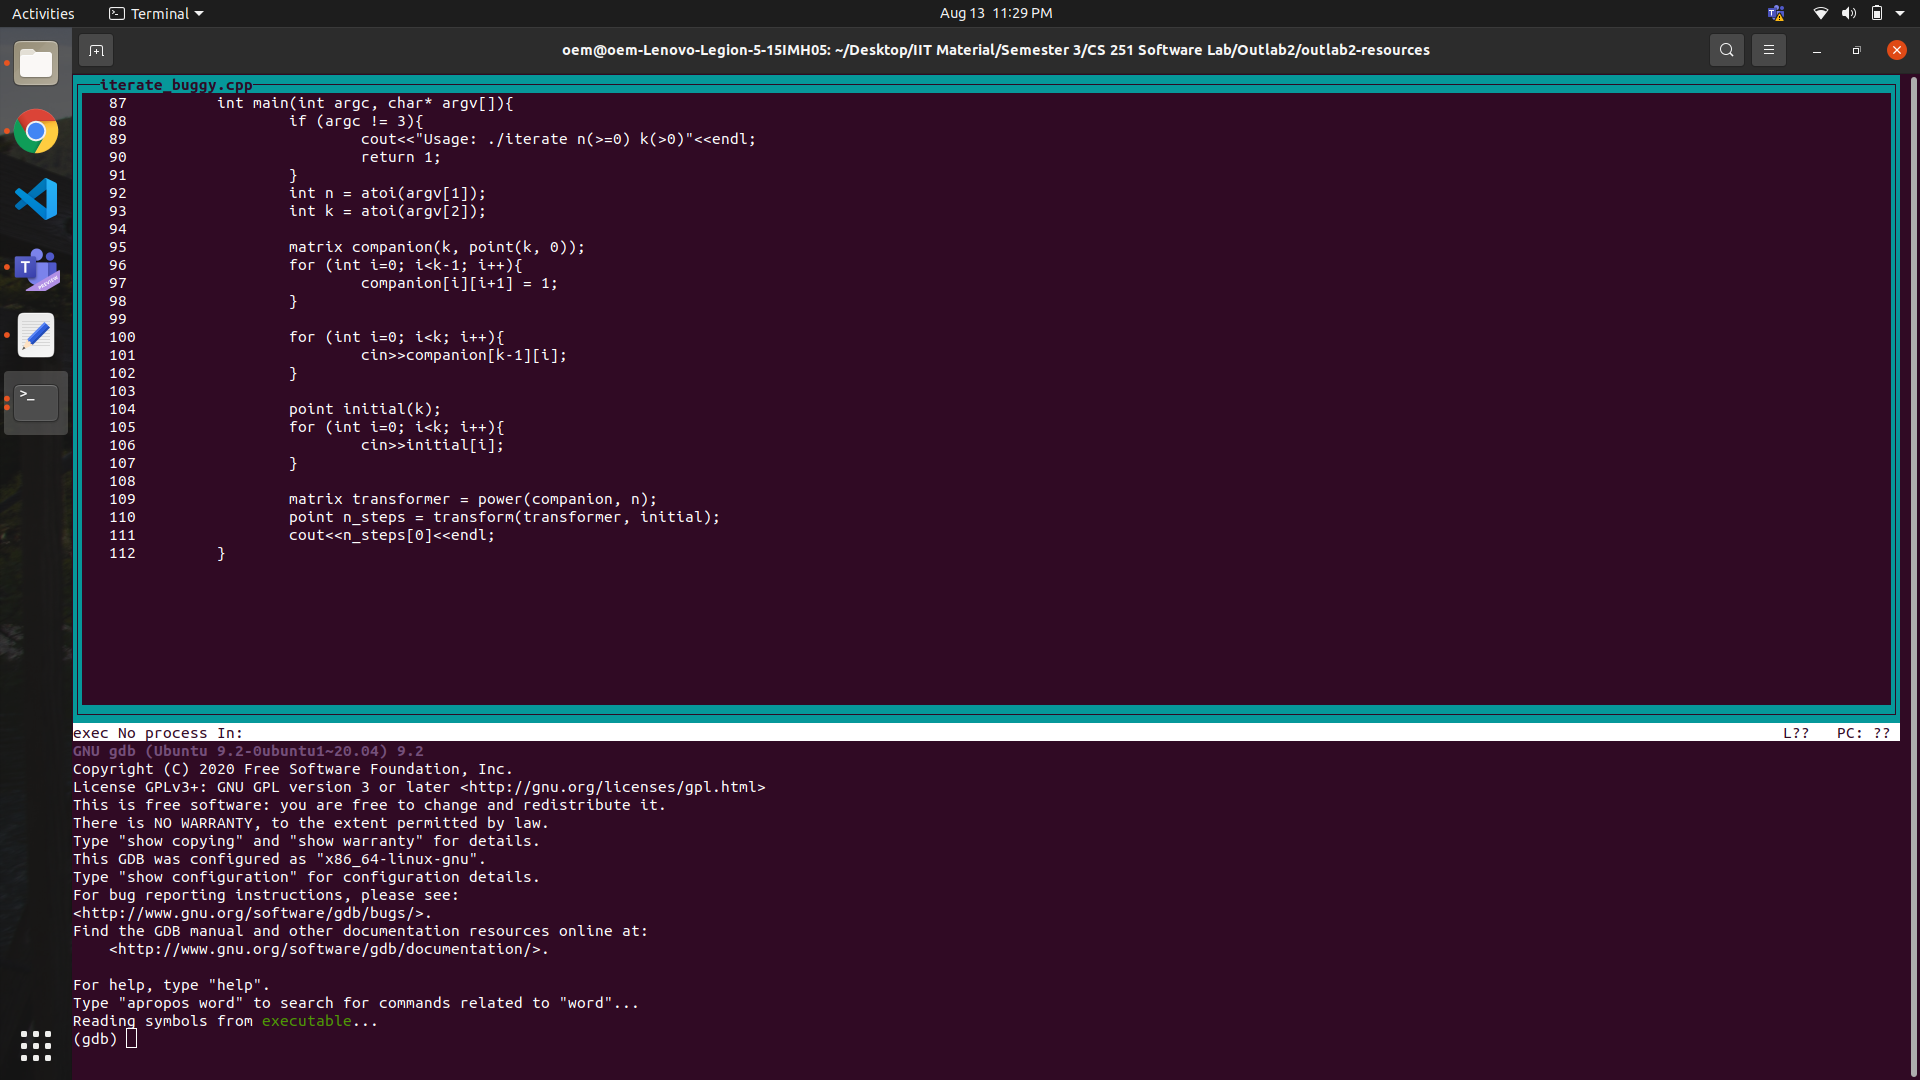
\includegraphics[width = \textwidth]{Screenshot1.png}
\caption{Screenshot1}
\label{fig:left}
\end{subfigure}
\begin{subfigure}{0.49\textwidth}
\centering
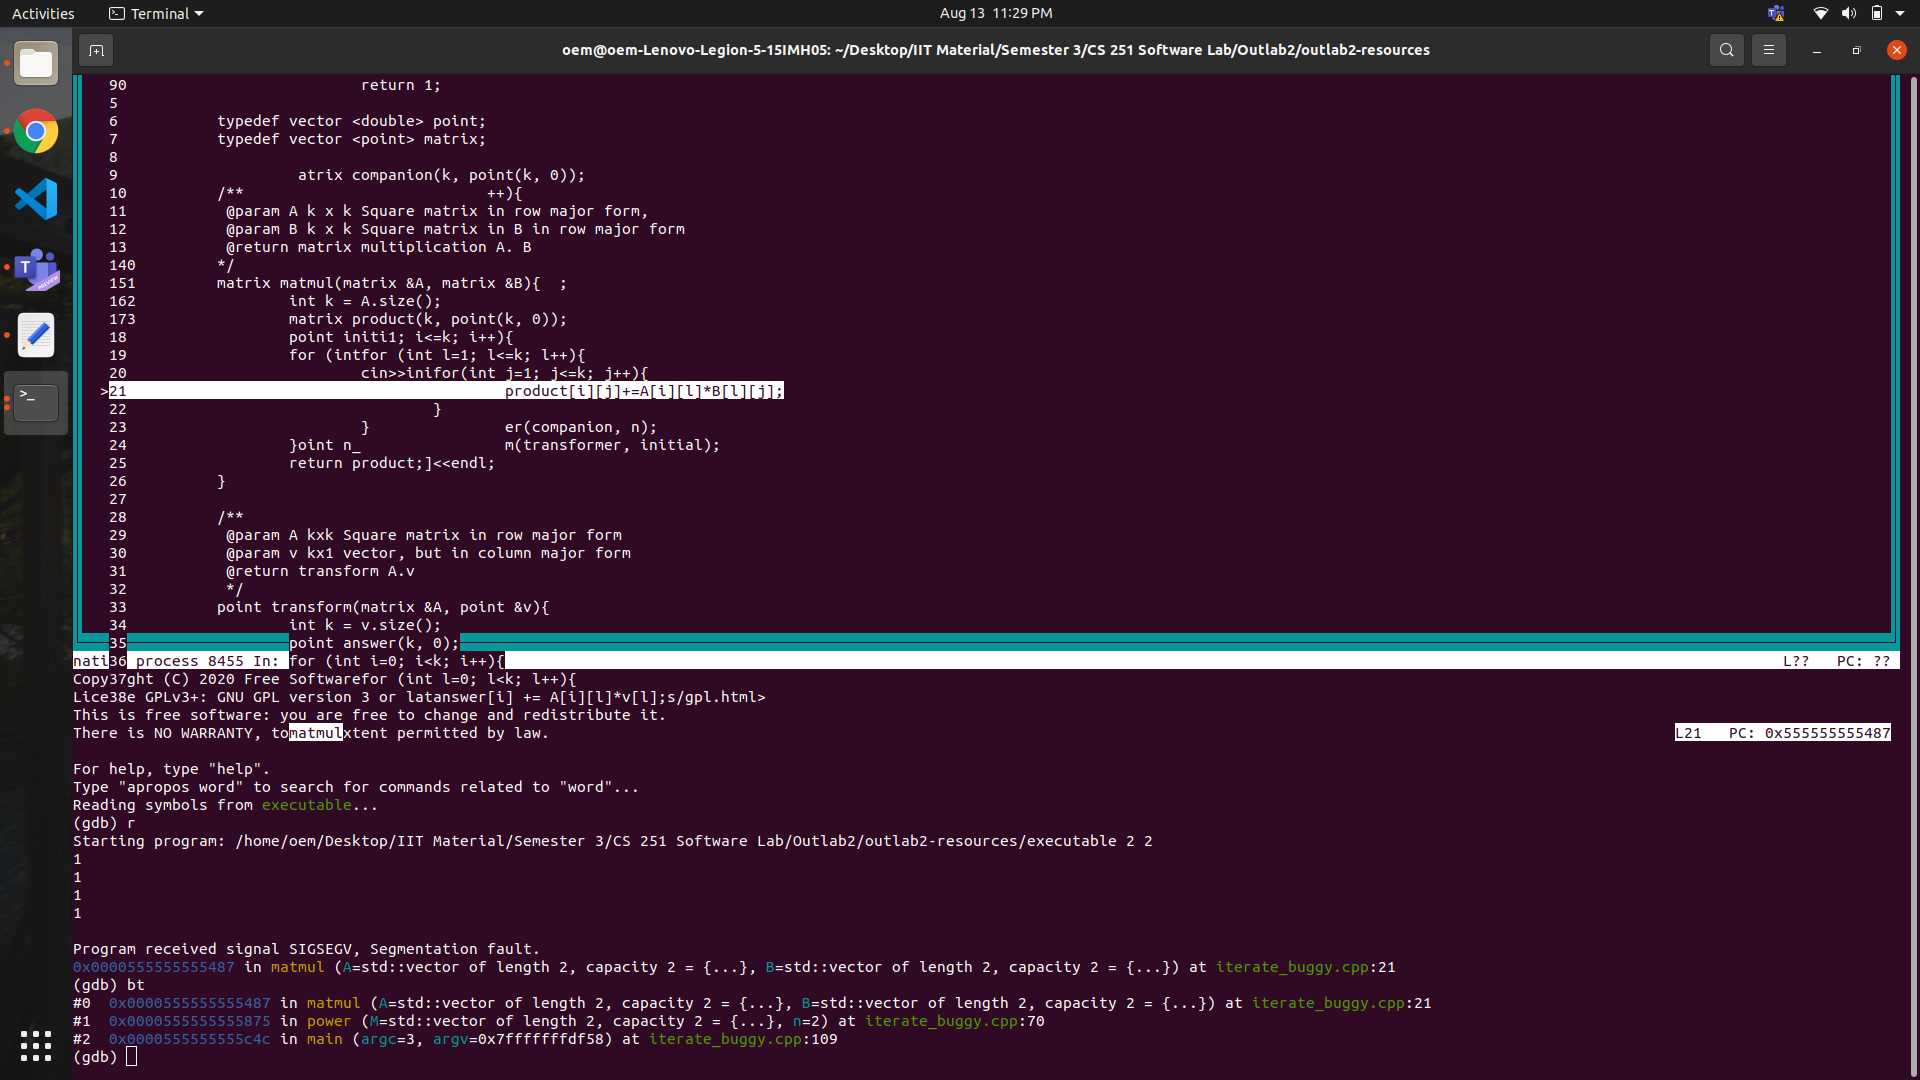
\includegraphics[width = \textwidth]{Screenshot2.png}
\caption{Screenshot2}
\label{fig:right}
\end{subfigure}
\caption{Combined figure}
\label{fig:combined}
\end{figure}
\clearpage


%table
\begin{table}
\centering
\begin{tabular}{ l | c }
\hline
 \textbf{operations} & \textbf{working}  \\ 
 \hline
 \{0, 0, 1, 0, 1, 0, 1, 1, 1\} & \{1, 0, 0, 1\}  \\  
 \hline
 \{0, 0, 1, 0, 1, 0, 1, 1\} & \{0, 1, 1, 1\} \\
 \hline
 \{0, 0, 1, 0, 1, 0, 1\} & \{1, 2, 2, 3\} \\
 \hline
 \{0, 0, 1, 0, 1, 0\} & \{8, 13, 13, 21\} \\
 \hline
 \{0, 0, 1, 0, 1\} &  \{233, 377, 377, 610\}  \\
 \hline
 \{0, 0, 1, 0\} & \{317811, 514229, 514229, 832040\} \\
 \hline
 \{0, 0, 1\} & \{365435296162, 591286729879, 365435296162, 591286729879\} \\
 \hline
 \{0, 0\} & \{7e+23,
    1e+24, 1e+24, 2e+24\} \\
 \hline
 \{0\} & \{2e+48,
    3e+48, 3e+48, 5e+48\} \\
 \hline
 \{\} & \{1e+97,
    2e+97, 2e+97, 4e+97\} \\
 \hline
\end{tabular}
\caption{Printing everything! Note the alignment}
\end{table}

\clearpage
\newpage 
\bibliographystyle{plainurl}
\bibliography{biblio}
\end{document}
 